\documentclass[12pt,a4paper,twoside]{book}

\usepackage[utf8]{inputenc}
\usepackage[english]{babel}

\usepackage[a4paper,inner=3.5cm,outer=2.5cm]{geometry}
\usepackage{parskip}
\usepackage{indentfirst}

\usepackage{graphicx}
\usepackage{float}
\usepackage{booktabs}
\usepackage{tabularx}
\usepackage{multirow}

\usepackage{natbib}
\bibliographystyle{ieeetr}
\setcitestyle{super,open={[},close={]}}

\usepackage{hyperref}

\usepackage{amsmath}
\usepackage{bm}

\usepackage[titletoc,title,toc,page]{appendix}
\usepackage{chngcntr}
\counterwithin{table}{chapter}
\usepackage[capitalize,noabbrev]{cleveref}

\usepackage{newlfont}
\usepackage{fancyhdr}
\usepackage{soul}
\usepackage{xcolor}
\usepackage{hyphenat}
\hyphenation{mate-mati-ca recu-perare}

\usepackage{enumitem}
\usepackage{listings}
\usepackage{verbatim}

\usepackage{tikz}
\usepackage{lscape}

\usepackage{tcolorbox}
\tcbuselibrary{skins, breakable}

\usepackage[font=footnotesize,labelfont=bf]{caption}

\newcommand{\rom}[1]{\uppercase\expandafter{\romannumeral #1\relax}}

\usepackage{pdfpages}

\lstset{
  aboveskip=1em,
  breaklines=true,
  captionpos=b,
  escapeinside={\%*}{*)},
  frame=single,
  numbers=left,
  numbersep=15pt,
  numberstyle=\tiny,
  basicstyle=\ttfamily\footnotesize
}

\definecolor{maroon}{cmyk}{0, 0.87, 0.68, 0.32}
\definecolor{halfgray}{gray}{0.55}
\definecolor{ipython_frame}{RGB}{207, 207, 207}
\definecolor{ipython_bg}{RGB}{247, 247, 247}
\definecolor{ipython_red}{RGB}{186, 33, 33}
\definecolor{ipython_green}{RGB}{0, 128, 0}
\definecolor{ipython_cyan}{RGB}{64, 128, 128}
\definecolor{ipython_purple}{RGB}{170, 34, 255}
\definecolor{outputcellbg}{RGB}{248,248,248}

\lstdefinelanguage{Python}{
    morekeywords={access,and,break,class,continue,def,del,elif,else,except,exec,finally,for,from,global,if,import,in,is,lambda,not,or,pass,print,raise,return,try,while},
    morekeywords=[2]{abs,all,any,basestring,bin,bool,bytearray,callable,chr,classmethod,cmp,compile,complex,delattr,dict,dir,divmod,enumerate,eval,execfile,file,filter,float,format,frozenset,getattr,globals,hasattr,hash,help,hex,id,input,int,isinstance,issubclass,iter,len,list,locals,long,map,max,memoryview,min,next,object,oct,open,ord,pow,property,range,raw_input,reduce,reload,repr,reversed,round,set,setattr,slice,sorted,staticmethod,str,sum,super,tuple,type,unichr,unicode,vars,xrange,zip,apply,buffer,coerce,intern},
    sensitive=true,
    morecomment=[l]\#,
    morestring=[b]',
    morestring=[b]",
    morestring=[s]{'''}{'''},
    morestring=[s]{"""}{"""},
    identifierstyle=\color{black}\ttfamily,
    commentstyle=\color{ipython_cyan}\ttfamily,
    stringstyle=\color{ipython_red}\ttfamily,
    keepspaces=true,
    showspaces=false,
    showstringspaces=false,
    rulecolor=\color{ipython_frame},
    frame=single,
    numbers=left,
    numberstyle=\tiny\color{halfgray},
    backgroundcolor=\color{ipython_bg},
    basicstyle=\scriptsize,
    keywordstyle=\color{ipython_green}\ttfamily,
}

\newtcolorbox{definition}[1][]{
    enhanced,
    breakable,
    colback=white,
    colframe=maroon,
    arc=2pt,
    boxrule=0.8pt,
    left=10pt,
    right=10pt,
    top=8pt,
    bottom=8pt,
    fonttitle=\bfseries,
    coltitle=white,
    title=Definition,
    #1
}

\newtcolorbox{example}[1][]{
    enhanced,
    breakable,
    colback=white,
    colframe=gray,
    arc=2pt,
    boxrule=0.8pt,
    left=10pt,
    right=10pt,
    top=8pt,
    bottom=8pt,
    fonttitle=\bfseries,
    coltitle=white,
    title=Example,
    #1
}

\begin{document}
\pagestyle{empty}
\newgeometry{left=2cm, right=2cm}
\begin{titlepage}
\begin{center}
    {{\Large{\textsc{Alma Mater Studiorum $\cdot$ Università di Bologna}}}}
    \rule[0.1cm]{\textwidth}{0.1mm}
    \rule[0.5cm]{\textwidth}{0.6mm}\\
    {\small{\bf Second Cycle Degree\\
    Artificial Intelligence}}
\end{center}

\vspace{45mm}

\begin{center}
    \textbf{Fundamentals of Artificial Intelligence \\ and Knowledge Representation \\ Module 1}
\end{center}

\vspace{60mm}
\par
\noindent
\begin{minipage}[t]{0.04\textwidth}
~
\end{minipage}
\begin{minipage}[t]{0.4\textwidth}
{{\textbf{Student:}\\
Matteo Canghiari}}
\end{minipage}
\begin{minipage}[t]{0.04\textwidth}
~
\end{minipage}

\vspace{30mm}

\begin{center}
    {\large{\bf Academic Year 2025/2026}}
\end{center}
\end{titlepage}

\restoregeometry

\pagestyle{empty}
\newpage~\newpage
\thispagestyle{empty}

\clearpage
\pagenumbering{arabic}
\pagestyle{plain}

\chapter{Searching for solutions}
Many AI problems can be solved by exploring the \textbf{solution space}. A solution space is a set of all the sequences of actions that an agent can apply. The agent examines all
the possible sequences of actions and chooses the best one. The goal is to reach the solution starting from a \textbf{initial state}. The process of trying different sequences
is called \textbf{search}. \vspace{3.5pt}

Usually, it's useful to think about the \textbf{search} process as a \textbf{search tree}, where:
\begin{itemize}
    \renewcommand{\labelitemi}{-}
    \item The initial state corresponds to the \textbf{root} of the tree.
    \item Each branch that makes up the tree defines the \textbf{action} that can performed by the current node.
    \item The nodes represent the subsequent reachable states. However, a certain node can be a \textbf{leaf node}. A leaf node is a new state to expand, a solution or a dead-end.
\end{itemize}
Previously, we said that a solution is a sequence of actions, so we need to define two main operations that allow us to build a sequence. We do this by \textbf{expanding}
the current state, applying each possible action to the current node, \textbf{generating} a new set of states\footnote{Every time we expand the current node, new state are generated.}.
Generally, the set of all leaf nodes available for expansion at any given point is called \textbf{frontier} or \textbf{fringe}. The process of expanding nods continues until
either a solution is found or there are no more states to expand. \vspace{3.5pt}

Finally, concluding this first introduction, we say that all the search algorithms are named \textbf{search strategies}, and typically they all share the same structure, varying
by the way they choose which state needs to be expand.
\label{c_1}

\section{Infrastructure for search strategies}
Every search strategy uses different kind of data structures to keep in mind how the search tree was built. Each node of the tree corresponds to a data structure, containing:
\begin{itemize}
    \renewcommand{\labelitemi}{-}
    \item State: the state in the state space.
    \item Parent: the node that generated this node.
    \item Action: the action taken by the parent to generate the node.
    \item Depth: defining how deep is the node, in which level it belongs to.
    \item Path-Cost: the cost of the path from the initial state to this node, usually denoted by $g(n)$.
\end{itemize}
Now that we have nodes, we need somewhere to put them. The fringe needs to be stored in such a way that the search algorithm can easily choose the next node to expand. The 
appropriate data structure is a \textbf{queue}. It can be a \textbf{FIFO}, \textbf{LIFO} or a \textbf{priority queue}\footnote{We remember that: 
    \begin{itemize}
        \setlength{\itemsep}{0pt}
        \renewcommand{\labelitemi}{-}
        \item LIFO queues pop the newest element.
        \item FIFO queues pop the oldest element.
        \item Priority queues pop the element with the highest priority.
    \end{itemize}
}.
\label{s_1_1}

\section{Measuring effectiveness}
This paragraph describes a new method to retrieve informations from data, named \textbf{probabilistic inference}.
It allows the computation of conditional probabilities for query propositions by given evidence.
Starting from an example is defined the \textbf{full joint distribution} as the knowledge base from which answers to all questions.
\begin{example}
  e.g. (\textit{Toothache, Cavity, Catch}) is just a domain consisting of three Boolean variables. \textit{Catch} condition occurs when the dentist's steel probe catches in the tooth. Based on the domain, the \textbf{full joint distribution} seems like this:
  \begin{center}
        \begin{table}[H]
            \centering
            \begin{tabular}{|c|c|c|c|c|}
                \hline
                \multicolumn{1}{|c|}{} & \multicolumn{2}{|c|}{\it toothache} & \multicolumn{2}{|c|}{\it $\neg$toothache} \\
                \hline
                \it & \it catch & \it $\neg$catch & \it catch & \it $\neg$catch \\
                \it cavity & 0.108 & 0.012 & 0.072 & 0.008 \\
                \it $\neg$cavity & 0.016 & 0.064 & 0.144 & 0.576 \\
                \hline
            \end{tabular}
            \caption{Full joint distribution of Toothache, Cavity and Catch}
            \label{t_1_2}
        \end{table}
    \end{center}
    The equation 
    \begin{center}
        $P(\phi) = \sum_{\omega:\omega\models\phi}P(\omega)$
    \end{center}
    gives a direct way to calculate probabilities of any assertions, summing up all the possible worlds that satisfy the original proposition. \vspace{3.5pt}

    e.g. $P(toothache) = 0.108 + 0.012 + 0.016 + 0.064 = 0.2$ 

    e.g. $P(cavity \vee toothache) = 0.108 + 0.012 + 0.072 + 0.008 + 0.016 + 0.064 = 0.28$

    It's also possible compute conditional probabilities: \vspace*{3.5pt}

    e.g. $P(\neg cavity|toothache) = \frac{P(\neg cavity \land toothache)}{P(toothache)} = \frac{0.016 + 0.064}{0.2} = 0.4$ \vspace{3.5pt}

    Notice that in this calculation the term $P(toothache)$ remains constant, no matter which value of \textit{Cavity} is computed. In fact, it can be viewed as a \textbf{normalization constant} $(\alpha)$ for the whole distribution $\mathbf{P}(Cavity|toothache)$, ensuring that the positive and negative case sum up to one, as the second probability axiom requires. \vspace*{7pt}

    $\mathbf{P}(Cavity|toothache) = \alpha\mathbf{P}(Cavity, toothache)$ \\
    $= \alpha[\mathbf{P}(Cavity, toothache, catch) + \mathbf{P}(Cavity, toothache, \neg catch)]$ \\
    $= \alpha[\langle0.108, 0.016\rangle + \langle0.012, 0.064\rangle]$ \\
    $= \alpha\langle0.12, 0.08\rangle = \langle0.6, 0.4\rangle$
\end{example}
\begin{definition}
    The first probability calculated $P(toothache)$ is called \textbf{marginalization}, or more simply \textbf{summing out}, because it sums up the probabilities for each possible value of the other variables.
\end{definition}
\begin{definition}
    The second one $P(\neg cavity|toothache)$ is named \textbf{conditioning}, a variant of marginalization that involves conditional probabilities instead of joint probabilities.
\end{definition}
\begin{definition}
    From the example, it's possible to extract a general inference procedure. Let \textbf{Y} be the query variables. Let \textbf{E} be the list of evidence variables, let \textbf{e} be the list of observed values for them, and let \textbf{H} be the unobserved variables. The \textbf{probability query} $\mathbf{P}(Y|\mathbf{e})$ defines the posterior joint distribution of a set of \textbf{query variables Y} given specific values \textbf{e} for some \textbf{evidence variables E}: \vspace{3.5pt}
    \begin{center}
        $\mathbf{P}(Y|e) = \alpha\mathbf{P}(Y, E=e) = \alpha\sum_{h}\mathbf{P}(Y, E=e, H=h)$
    \end{center}
\end{definition}
The full joint distribution can answer probabilistic queries for discrete variables, but only for small domains. It does not scale well: for a domain described by \textit{n} Boolean variables, it requires an input table of size \textit{$O(2^n)$} and takes \textit{$O(2^n)$} time to process a question. The full joint distribution in tabular form is just not a practical tool for building reasoning systems.
\label{s_1_2}

\chapter{Non-informed strategies}
This chapter covers several search strategies that come under the heading of \textbf{non-informed strategies}. The term \textit{non-informed} means that the strategies have no 
additional knowledge about the domain; all they can do is generate successors and distinguish a goal state from a non-goal state. We introduce five non-informed search strategies:
\begin{itemize}
    \renewcommand{\labelitemi}{-}
    \item BFS.
    \item Uniform-cost search.
    \item DFS.
    \item DFS with limited depth.
    \item Iterative deepening.
\end{itemize}
\label{c_2}

\section{Breadth-first search}
\textbf{Breadth-first search} is a simple strategy in which the root node is expanded first, then all the successors of the root node are expanded next, and so on; until it is
found the goal-state or the goal-node. \vspace{3.5pt}

At algorithmic level, this is achieved very simply using a FIFO queue for the fringe, so the oldest node will be the first expanded. Before generating, so creating new states,
the goal-test is applied to the \textbf{shallowest} node. \vspace{3.5pt}

This strategy ensures \textbf{completeness}, but the \textbf{shallowest} goal node is not necessary the \textbf{optimal} one. BFS can be optimal if all the actions have the same 
path-cost. In addition, breadth-first search seems to take a quite huge of time and memory. Suppose a search tree where every node has $b$ successors. The root node generates
$b$ nodes at the first level, each of which generates $b$ more successors, for a total of $b^2$ nodes. Now if we consider that the goal-node has $d$ depth, in the worst case 
the total number of nodes generated is \vspace{3.5pt}
\begin{center}
    $b + b^2 + b^3 + \dots = O(b^d)$.
\end{center} \vspace{3.5pt}
This complexity is the same for both time and memory. As the time complexity, the memory takes into account every node expanded inside the \textbf{explored set} to avoid
\textbf{loopy path}; the space complexity grows exponentially with the number of $b$ successors and the depth $d$ of the goal node. The problem of memory seems to be the most serious. \vspace{3.5pt}

In general, any exponential complexity seems to be scary, and in this case uninformed strategies cannot solve massive problems.
\label{s_2_1}

\section{Uniform-cost search}
The previous paragraph noted the importance of absolute and conditional independence relationships in simplifying probabilistic representation.
This section introduces a systematic way to represent such relationships in the form of \textbf{Bayesian networks}.
We define the syntax and semantics of these networks and show how they can be used to capture uncertain knowledge. \vspace{7pt}

A Bayesian network is a simple graphical notation for conditional independence assertions and hence for a compact specification of full joint distribution.
The Bayesian network's syntax is composed by:
\begin{enumerate}
    \item Each node corresponds to a random variable.
    \item A set of directed links or arrows connects pairs of nodes.
    \item Each node $X_i$ has a conditional probability distribution $\mathbf{P}(X_i|Parents(X_i))$, that quantifies the effect of the parents on the node.
\end{enumerate}
\begin{example}
    i.e. Topology of network encodes conditional independence assertions: \vspace{3.5pt}
    \begin{center}
        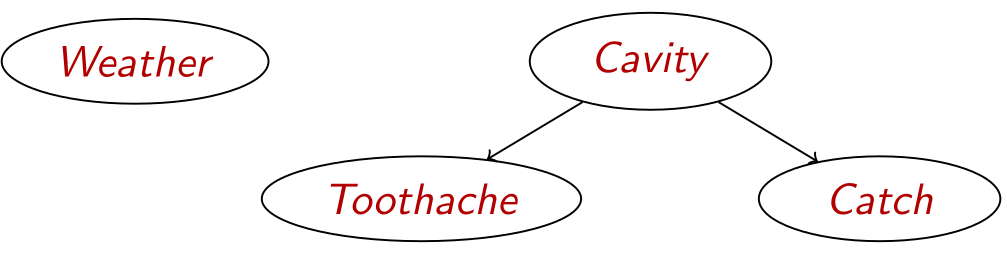
\includegraphics[width=0.6\textwidth]{img/img2.png}
    \end{center} \vspace{3.5pt}
    \begin{itemize}
        \renewcommand{\labelitemi}{-}
        \item Weather is independent of the other variables\footnote{Formally, the absolute or conditional independence is indicated by the absence of a link between nodes.}.
        \item Toothache and Catch are conditionally independent given Cavity\footnote{The intuitive meaning of an arrow is typically that X has a direct influnce on Y, which suggests that causes should be parents of effects.}.
    \end{itemize}
\end{example}
\begin{example}
    i.e. I'm at work, neighbor John calls to say my alarm is ringing, but neighbor Mary doesn't call. Sometimes it's set off by minor earthquakes. Is there a burglar? \vspace{3.5pt}

    The random variables are: \it Burglar, Earthquake, Alarm, MaryCalls, JohnCalls \footnote{The network topology reflects \textbf{causal} knowledge, from the causes nodes we define the effects nodes.}\footnote{For each node the conditional distribution are shown as a \textbf{conditional probability table}, or simply CPT.}\footnote{Let's take a look at the tables. In this network we are talking about joint distribution, not full joint distribution. Simply, the full joint distribution about boolean random variables can be computed by $1-P(a)$.}. \vspace{3.5pt}
    \begin{center}
        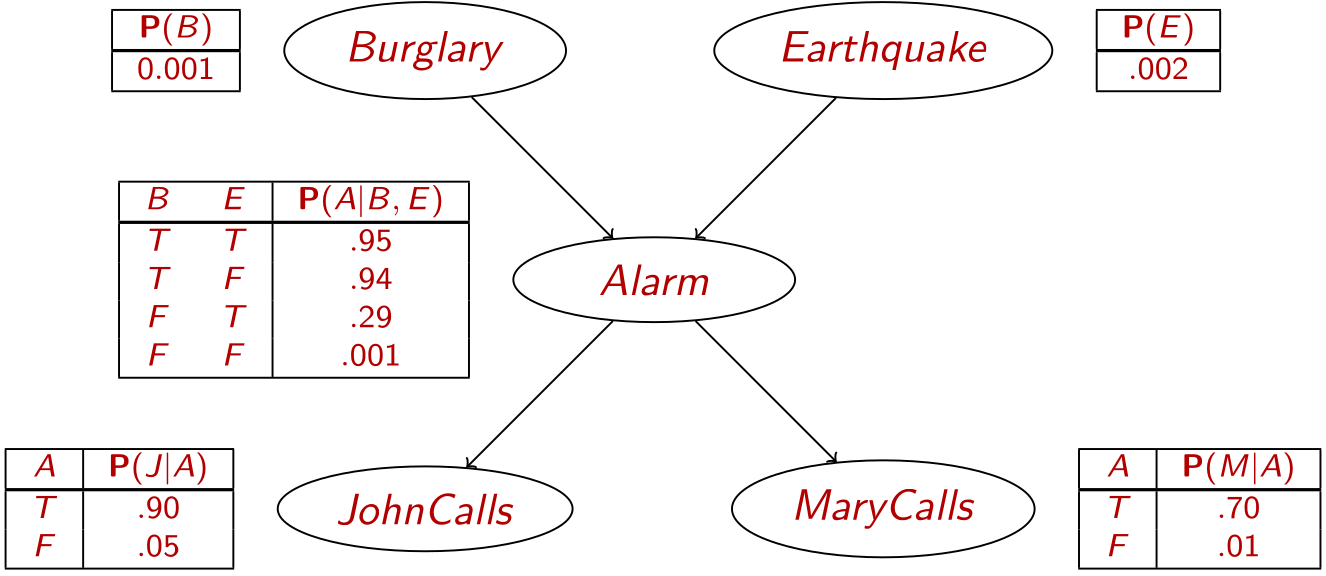
\includegraphics[width=0.75\textwidth]{img/img3.png} \vspace{3.5pt}
    \end{center}
\end{example}

We begin the discussion with a simple toy example, the \textit{student network}.
\begin{example}
    i.e. A student's grade depends on intelligence and on the difficulty of the course.
    SAT scores are correlated with intelligence. A professor writes recommendation letters by only looking at grades. \vspace{3.5pt}

    In this case, our probability space is composed by five relevant random variables: \textit{Difficulty (D)}, \textit{Intelligence (I)}, \textit{SAT score (S)}, \textit{Grade (G)} and \textit{Letter (L)}. \vspace{3.5pt}
    \begin{center}
        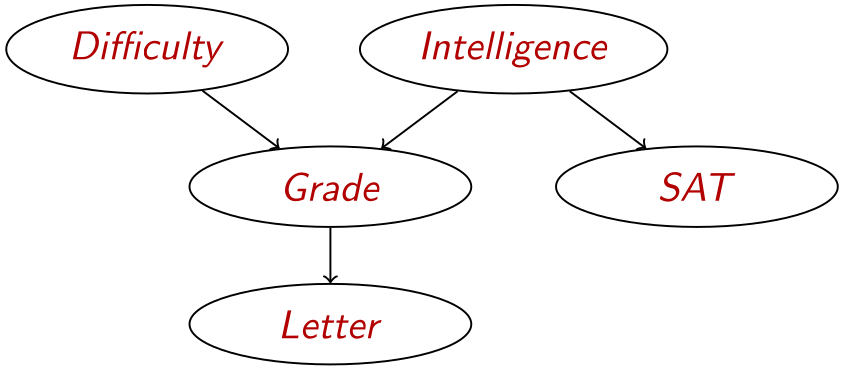
\includegraphics[width=0.5\textwidth]{img/img4.png}
    \end{center} \vspace{3.5pt}
    Consider a particular student, George, that he would like to reason using the student network. We might ask how likely George is to get a strong recommendation from his professor in Analysis.
    Knowing nothing else about George and his grade, this probability is around the $50$ percent. \vspace{3.5pt}

    We now find out that George is not so intelligent. The probability that he gets a strong letter from the professor goes down to 39. We now further discover that Analysis is an easy class.
    The probability that George receive a strong letter is now about 51 percent. \vspace{3.5pt}

    Queries and answers such as this, where we predict the behaviors from causes to effects, are called \textbf{causal reasoning} or \textbf{prediction}\footnote{It reflects the causal direction, from the parent nodes we are just defining which is their influence on their children.}. \vspace{3.5pt}

    Now, assume a recruiter, trying to hire George based on our previous model. By a prior probability, the recruiter believes that George is 30 percent likely to be intelligent. 
    He obtains George's grade record for the class Analysis and sees that George received a low score in that class. His probability that George has high intelligence goes down,
    about 7.9 percent. We note that the probability that the class is a difficult one also goes up, from 40 percent to 62.9 percent. Now, consider that the recruiter lost George's trascript of records, and has only the recommendation letter from George's professor in Analysis, which is weak.
    The probability that George has high intelligence still goes down, but only to 14 percent. Note that if the recruiter has both the grade and the letter, we have the same probability
    as if he had only the grade. \vspace{3.5pt}

    Queries such as this, where we reason from effects to causes, are named \textbf{evidential reasoning} or \textbf{explanation}\footnote{In this case, we are not reasoning from top to bottom, but instead from bottom to top.}. \vspace{3.5pt}

    Finally, George submits his high SAT score to the recruiter. The probability that George has high intelligence goes up dramatically, from 7.9 percent to 57.8 percent. Intuitively, the reason that the SAT score 
    outweights the poor grade is that a student with low intelligence are unlikely to get good scores on their SAT, whereas students with high intelligence can still get C grades in hard class.
    Indeed, we see that the probability that Analysis is a difficult one goes up from 62.9 percent to 76 percent. \vspace{3.5pt} 

    This last pattern is a interesting one. The information about SAT score told us other informations about the student's intelligence, which, in conjuction with the student's grade, gave us some clues about the difficulty of the course. Let examine this pattern in probabilistic terms. \vspace{3.5pt}

    We are saying \vspace{3.5pt}

    $P_s(i^1|g^3) = 0.079$ \vspace{3.5pt}

    On the other hand, if we consider that Analysis is a hard class, we have \vspace{3.5pt}

    $P_s(i^1|d^1, g^3) = 0.11$ \vspace{3.5pt} 

    Here, we are partially explaining why George has got a poor grade. By the way, taking a more tricky example, for instance George got a middle grade in Analysis, we have that \vspace{3.5pt}

    $P_s(i^1|g^2) = 0.175$ \vspace{3.5pt}

    Also if Analysis is a hard class, we get \vspace{3.5pt} 

    $P_s(i^1|d^1, g^2) = 0.34$ \vspace{3.5pt} 

    In effect, we have justified the poor grade via the difficulty of the class. Explaining away is an instance of a general pattern called \textbf{intercasual reasoning},
    where different causes of the same effect, so they are parents of the effect node, can interact.     
\end{example}
\textbf{Compactness} \vspace{3.5pt}

A Bayesian network can often be more \textit{compact} than the full joint distribution. The \textbf{compactness} of a Bayesian network is a property that makes easy to handle
domain with many random variables. \vspace{3.5pt}

At the same time, a Bayesian network grows \textit{linearly}, instead of an \textit{exponential} growth by full joint distribution. Assuming a domain composed by $\mathbf{n}$ Boolean
variables, where each of them is associated with a CPT \textit{(Conditional Probability Table)}\footnote{A CPT for a Boolean variable $\mathbf{X_i}$ with $\mathbf{k}$ parents, has $\mathbf{2^k}$
rows for the combinations of parents values and usually is defined only the True case; the negative case, however $X_i = False$, can be simply computed by the third probability axiom $\mathbf{1 - p}$.}.
If each variable has no more then $\mathbf{k}$ parents, the complete network requires $O(n \times 2^k)$ numbers, as we already know to complete the full joint distribution are necessary
$O(2^n)$.
\begin{example}
    i.e. Comparison of parameters required from the previously example between Bayesian network and full joint distribution. \vspace{3.5pt}

    For the burglar network: \vspace{3.5pt}

    $1 + 1 + 4 + 2 + 2 = 10$ numbers required by the Bayesian network \vspace{3.5pt}

    $2^5 - 1 = 47$ numbers required by the full joint distribution
\end{example}
\textbf{Global semantics} \vspace{3.5pt}

A Bayesian network is a directed acyclic graph with some numeric parameters attached to each node. One way to define what the network means is to define the way in which 
it rapresents a full joint distribution. 
\begin{definition}
    \textbf{Global semantics} defines the full joint distribution as the product of the local conditional distributions:
    \begin{center}
        $P(x_1, ..., x_n) = \prod_{i = 1}^{n} P(x_i|parents(X_i))$
    \end{center}
\end{definition}
\begin{example}
    i.e. 
    
    $P(j, m, a, \neg b, \neg e) \\
    = P(j|a)P(m|a)P(a|\neg b \wedge \neg e)P(\neg b)P(\neg e) \\
    = 0.9 \times 0.7 \times 0.001 \times 0.999 \times 0.998 = 0.000628$
\end{example}
\textbf{Flow of influence} \vspace{3.5pt}

Until now, we used the intuition that edges represent direct dependence. For instance, we said that the letter recommendation from the professor depends only on the student's grade;
this state was encoded by the fact that there is an exit edge from \textit{G} that arrive to \textit{L}. This intuition is \textbf{not} always true. \vspace{3.5pt}

The aim of this section is to understand when we can guarantee independence between random variables. First of all, we begin with a simple case analysis: we try to understand
when a variable \textbf{X} can influence \textbf{Y} given \textbf{Z}. \vspace{3.5pt}

\textbf{Direct connection}. This is the simple case, when X and Y are directly connected via an edge. If X and Y are directly connected, we can always get examples where they 
influence each other, regardless of \textbf{Z}. \vspace{3.5pt}

\textbf{Indirect connection}. Now  we are considering the more complicated case when X and Y are not directly connected, but there is a trail between them. There are four cases
where X and Y are connected via Z. \vspace{3.5pt}
\begin{center}
    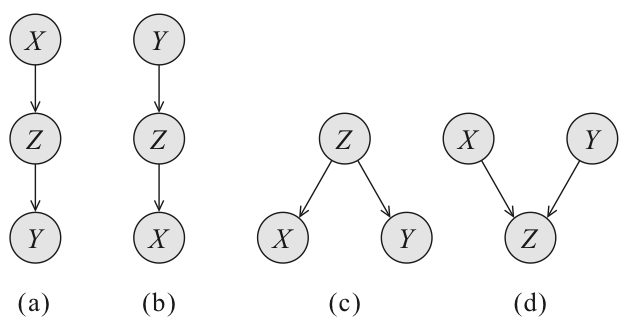
\includegraphics[width=0.6\textwidth]{img/img5.png}
\end{center} \vspace{3.5pt}
The first two correspond to causal chains, the third to a common cause, and the last one to a common effect.

\textbf{(a) Causal trail}. We have a chain like $X \rightarrow Z \rightarrow Y$. X cannot influence Y via Z if Z is observed.

\textbf{(b) Effect trail}. Now we have the same trail but in the opposite direction, so  $Y \rightarrow Z \rightarrow X$. Another time, Y cannot influence X via Z if Z is observed.

\textbf{(c) Common cause}. This type of trail defines the same grade of independence as before. If Z is observed then neither X or Y can influence each other. 

\textbf{(d) Common effect}. In the previously cases, we see a common pattern: if Z is observed then neither X or Y can influence each other. By the way, this kind of trail, 
$X \rightarrow Z \leftarrow Y$, has a new behavior. If Z is not observed influence cannot flow along the trail. So if Z is observed X and Y are independent. In the student example
we analyzed this case, which we called \textit{intercausal reasoning}; we showed that the probability that student has high intelligence goes down when we observe that his grade is 
a poor score, but then goes up when we observe that the class is a hard one. Let us consider a variant of the same case. Assume that we do not observe the student's grade, but we observed
that he received an awful recommendation letter. Intuitively, the same phenomenon happens. The weak letter told us that he received a low grade, and it is sufficient to 
correlate Intelligence and Difficulty.  
\begin{definition}
    If influence can flow from X to Y via Z, the trail $X \longleftrightarrow Z \longleftrightarrow Y$ is \textbf{active}.
\end{definition}
If we consider a longer trail $X_1 \rightarrow \dots \rightarrow X_n$, the first variable $X_1$ can influence the last variable $X_n$, if influence can flow through every single node of the trail.
This will be true if and only if every two-edge trail $X_{i-1} \longleftrightarrow X_i \longleftrightarrow X_{i+1}$ along the trail allows influence to flow.
\begin{definition}
    Let \textbf{Z} be a subset of observed variables. The trail $X_{i-1} \longleftrightarrow X_i \longleftrightarrow X_{i+1}$ is \textbf{active given} Z if
    \begin{itemize}
        \renewcommand{\labelitemi}{-}
        \item $\forall X_{i-1} \rightarrow X_i \leftarrow X_{i+1}$, $X_i$ or one of its descendants are in Z\footnote{The trail reported is the common effect case.}
        \item no other node along the trail is in Z
    \end{itemize}
\end{definition}
However, inside the Bayesian network literacy there is another important notion, named \textbf{d-separation}.
\begin{definition}
    Two sets of nodes \textbf{X}, \textbf{Y} are d-separated given Z if there is no active trail between any $X \in \mathbf{X}$ and $Y \in \mathbf{Y}$ given \textbf{Z}.
\end{definition}
It's possible to summarize few steps to follow to determine if X and Y are independent given Z:
\begin{enumerate}
    \item Mark all nodes in Z or having descendants in Z.
    \item Traverse the graph from X to Y, stopping if we get to a \textbf{blocked} node\footnote{A node is blocked if that node is the middle of an unmarked v-structure \textit{(common effect case)}, or belongs to Z \textit{(cannot be both).}}.
    \item If we can't reach Y, then X and Y are independent.
\end{enumerate}
Another aspects about independence are introduces by the meaning of \textbf{local semantics} and \textbf{Markov blanket}.
\begin{definition}
    \textbf{Local semantics} define that each node is conditionally independent of its \textbf{non-descendants} given its parents\footnote{Here, we are considering the parents of the first node, not the parents of non-descendants.}. 
\end{definition}
\begin{definition}
    Each node is conditionlly independent of all the others nodes given its \textbf{Markov blanket}: so its parents, children and children's parents.
\end{definition}
\label{s_2_2}

\section{Depth-first search}
\textbf{Depth-first search} always expands the \textit{deepest} node in the current fringe. The search proceeds immediately to the deepest level of the the search tree, where
the nodes have no successors. As those nodes are expanded, they are dropped from the fringe, so the search \textbf{goes back} to the next deepest node,
which is located at $m - 1$ depth of the current nodes deleted from the frontier. \vspace{3.5pt}

While BFS uses a FIFO queue, DFS uses a LIFO queue, the most recently generated node is chosen for expansion. This search strategy ensures \textbf{optimality} but not 
\textbf{completeness}, for instance, in the figure shown below the algorithm will follow $Arad-Sibiu-Arad-Sibiu$ loop forever. However, the search tree can be modified at no-extra
memory cost: DFS checks new generated states against those on the path from the root to the current node. This avoids infinite loops, but does not guarantees the proliferation
of redudant paths. \vspace{3.5pt}
\begin{center}
    % \includegraphics{95/1152}
\end{center}

Compared to BFS, depth-first search has one major advantage, the space complexity; for any search tree, it needs to store only a single path from the root to a leaf node. Given 
a branch factor $b$ and a maximum depth $m$, DFS requires storage of only $O(bm)$ nodes. Even if the space complexity seems to be linear, in the worst case the time complexity
reaches the exponential order\footnote{We remind you that the maximum depth $m$ can be bigger than the shallowest depth $d$, introduced in the breadth-first search strategy.}.
\label{s_2_3}

\section{Depth-limited search}
As we said, depth-first search is not complete: the algorithm could enter in infinite cycles. This problem can be avoided introducing some changes to the original algorithm, such as
a predetermined depth limit $l$. All the nodes at depth $l$ are treated as leaves node, they have no successors. This search strategy is called \textbf{depth-limit search}.
Unfortunately, even though it solves the problem of infinite cycles, it introduces another source of \textbf{no-completeness}; if we choose a limit $l < d$, the shallowest goal-node
may not be achieved. Depth-limited search will also be \textbf{non-optimal} if we choose $l > d$. \vspace{3.5pt}

It's time complexity is exponential, $O(b^l)$, and its space complexity is linear, $O(bl)$\footnote{Depth-first search can be viewed as a special case of depth-limit search with $l=\infty$}.
\label{s_2_4}

\section{Iterative deepening}
\textbf{Iterative deepening search} is a strategy usually used with the depth-first search algorithm, which defines iteratevely the \textit{best depth limit}. It does this by 
gradually increasing the limit $l$, as we have seen in depth-limited search, until the target node is found. This will occur when the depth limit $l$ reaches $d$, the depth of the
shallowest node. \vspace{3.5pt}

It combines the advantages of depth-first search and breadth-first search strategies. Like DFS, its memory complexity is linear, to be precise $O(bd)$\footnote{Iterative deepening search, such as the depth-first search, only maintains in memory one path at the time; it is discarded if it does not contains the goal node.}. 
Like BFS, it is \textbf{complete} when the brancing factor $b$ is finite and \textbf{optimal} when the path cost increases as a function of the node depth. \vspace{3.5pt}

Iterative deepening may seem like a waste of computation because the initial nodes are generated multiple times, but the execution time never gets worsen. The reason 
is that in a search tree with the same branching factor at each level, most of the nodes are in the bottom level, so it does not matter much that the upper levels are generated
multiple times. Let's consider an example for better understanding.
\begin{example}
    i.e. Considering the branching factor equal to 10 and the depth of the shallowest node equal to 5, briefly: \vspace{3.5pt}
    \begin{center}
        \begin{itemize}
            \renewcommand{\labelitemi}{}
            \item $b = 10$
            \item $d = 5$
        \end{itemize}
    \end{center} \vspace{3.5pt}

    and given the equation which defines the total number of nodes generated by iterative deepening in the worst case \vspace{3.5pt}
    \begin{center}
        $N(IDS) = (d)b + (d - 1)b^2 + \dots + (1)b^d$        
    \end{center} \vspace{3.5pt}

    we have \vspace{3.5pt}
    \begin{center}
        $N(IDS) = 50 + 400 + 3.000 + 20.000 + 100.000 = 123.450$        
    \end{center} \vspace{3.5pt}

    while we could get the same amount if we decide to use breadth-first search strategy \vspace{3.5pt}
    \begin{center}
        $N(BFS) = 10 + 100 + 1.000 + 10.000 + 100.000 = 111.110$        
    \end{center} \vspace{3.5pt}
\end{example}
\label{s_2_5}

\section{Summary of Non-informed strategies}
\begin{center}
    \begin{tabular}{|l|c|c|c|c|c|}
        \hline
        \bf Criterion & BFS & UCS & DFS & DLS & IDS \\
        \hline
        \bf Time & $O(b^d)$ & $O(b^d)$ & $O(b^m)$ & $O(b^l)$ & $O(b^d)$ \\
        \hline
        \bf Space & $O(b^d)$ & $O(b^d)$ & $O(bm)$ & $O(bl)$ & $O(bd)$ \\
        \hline
        \bf Optimal & No & Yes & Yes & No & Yes \\
        \hline
        \bf Complete & Yes & Yes & No & Yes if $l \ge d$ & Yes \\
        \hline
    \end{tabular}
\end{center}
\footnote{Comparison of Breadth-first search, Uniform-cost search, Depth-first search, Depth-limited search and Iterative deepening search.}
\label{s_2_6}

\chapter{Informed strategies}
This paragraph shows how \textbf{informed search strategies} can find solutions more efficiently than \textbf{non-informed search strategies}.

The general approach about informed search strategies is defined by \textbf{best-first search strategy}. Best-first algorithm select a node for the expansion based on an 
\textbf{evaluation function}, briefly written as $f(n)$. Generally, this type of search strategy uses evaluation function as an estimation of the effort required to reach the 
final state; the node with the lowest evaluation is expanded first. \vspace{3.5pt}

The choice of the evaluation function $f(n)$ determines the search strategy. Most best-first algorithms include as a component of $f(n)$ a \textbf{heuristic function}, denoted
$h(n)$. \vspace{3.5pt}
\begin{center}
    $h(n) =$ estimated cost of the path from the current node $n$ to the final state\footnote{Until now, we saw the $g(n)$ function as the path cost from the root node to the
    current state; selecting the node for the expansion with the lowest $g(n)$. Instead the heuristic function $h(n)$ defines the distance from the current node to the final state!}.
\end{center}
We will examine two main applications of the best-first search strategy, which are:
\begin{itemize}
    \renewcommand{\labelitemi}{-}
    \item Greedy best-first search.
    \item A* search.
\end{itemize} 
\label{c_3}

\section{Greedy best-first search}
\textbf{Greedy best-first search} tries always to expand the node closest to the goal state, in a such a way it wanted to build the path that leads to the quickest solution. Thus,
it evaluates nodes by using just the \textit{heuristic function}, $h(n)$. In this case, the \textit{evaluation function} is equal to the \textit{heuristic function}, $f(n) = h(n)$. \vspace{3.5pt}

Let's see how this works for the Romania graph example\footnote{Remember that is always possible to make a tree from a graph, and vice versa.}.
\begin{example}
    i.e. Romania graph, starting from Arad and arriving in Bucharest.
    \begin{center}
        % \includegraphics{Romania graph or tree}
    \end{center}
    We use the \textbf{straight-line distance} heuristic, which we will briefly call $h_{SLD}$. Given Bucharest as the goal state, we must know the straight-line 
    distances to Bucharest. For instance,
    $h_{LSD}(Arad) = 366$. The table below shows each straight-line distance from any given node to Bucharest. \vspace{3.5pt}

    \begin{center}
        \begin{tabular}{|l|p{2cm}|l|p{2cm}|}
            \hline
            \bf Arad & 366 & \bf Mehadia & 241 \\
            \hline
            \bf Bucharest & 0 & \bf Neamt & 234 \\
            \hline
            \bf Craiova & 160 & \bf Oradea & 380 \\
            \hline
            \bf Drobeta & 242 & \bf Pitesti & 100 \\
            \hline
            \bf Eforie & 161 & \bf Rimnicu Vilcea & 193 \\
            \hline
            \bf Fagaras & 176 & \bf Sibiu & 253 \\
            \hline
            \bf Giurgiu & 77 & \bf Timisoara & 329 \\
            \hline
            \bf Hirsova & 151 & \bf Urziceni & 80 \\
            \hline
            \bf Iasi & 226 & \bf Vaslui & 199 \\
            \hline
            \bf Lugoj & 244 & \bf Zerind & 374 \\
            \hline
        \end{tabular}
    \end{center} \vspace{3.5pt}

    Given the table, the first node to be expanded from Arad will be Sibiu, because it is closer to Bucharest than either Zerind or Timisoara. The next node to be expanded
    will be Fagaras because it is closest. Fagaras generated Bucharest, which is the goal. For this problem, greedy best-first search, using the heuristic $h_{LSD}$, finds 
    a solution without ever expanding a node that is not on the solution path. \vspace{3.5pt} 

    \begin{center}
        $\langle Arad, Sibiu, Fagaras, Bucarest\rangle = 450$
    \end{center} \vspace{3.5pt}

    However, the proposed solution is not optimal: the path via Sibiu, Rimnicu Vilcea, Pitesti and Bucharest is lower than the first one. \vspace{3.5pt}

    \begin{center}
        $\langle Arad, Sibiu, Rimnicu, Pitesti, Bucharest\rangle = 418$
    \end{center} \vspace{3.5pt}
\end{example}
This example shows why the algorithm is called \textbf{greedy}, at each step it tries to get as close to the goal as it can. By the way, this search strategy is \textbf{non-optimal}
and may be \textbf{incomplete}, if the data structure presents loopy path. \vspace{3.5pt}

In the worst case, if the depth of the shallowest node is $d$ and the branching factor is $b$, either the time and space complexity will be exponential, $O(b^d)$.
\label{s_3_1}

\section{A* search}
Even if the number of parents k is smallish, fill any CPT requires $O(2^k)$ numbers and it grows exponentially with number of parents. Instead, if we assume a 
continuous-valued parent or child, CPT becomes \textbf{infinite} \footnote{One of the nicest thing of Bayesian network is the capability to combine together
different types of variables, sush as descrete, continuos, deterministic, not-deterministic and so on.}. Usually, a solution to solve these types of
problem consists of \textbf{canonical distributions}. \vspace{3.5pt}

The simplest case is provided by \textbf{deterministic nodes}:
\begin{center}
    $X = f(Parents(X))$
\end{center}
A deterministic node has its values specified exactly by the values of its parents, with no uncertainty.
\begin{example}
    i.e. Logical relationship, so there is no stochasticity. \vspace{3.5pt}

    The relationship between the parent nodes $(Canadian, US, Mexico)$ and the child node $(NorthAmerican)$ is simply that the child is the disjunction, or the logical OR,
    of the parents. \vspace{3.5pt}

    \begin{center}
        \begin{tabular}{|c|c|c|c|}
            \hline
            \bf Canadian & \bf US & \bf Mexico & \bf NorthAmerican  \\
            \hline
            F & F & F & F \\
            T & F & F & T \\
            F & T & F & T \\
            F & F & T & T \\
            T & T & F & T \\
            T & F & T & T \\
            F & T & T & T \\
            T & T & T & T \\
            \hline
        \end{tabular}
    \end{center} \vspace{7pt}

    i.e. Numerical relationship. \vspace{3.5pt}
    
    If the parent nodes are a lake's inflows $(Rivers, Runoff, Precipitation)$ and the outflows $(Rivers, Evaporation, Seepage)$ and the child node is the
    change in the water level of the lake, then the value of the child is the sum of the inflow parents minus the sum of the outflow parents. \vspace{3.5pt}

    \begin{center}
        $\frac{Level}{t}=inflow+precipitation-outflow-evaporation$
    \end{center}
\end{example}

Another interesting example is the \textbf{Noisy-OR distribution}, which is very useful representation. Now, we will describe an example to understand the intuition
of Noisy-OR distribution given a medical domain.
\begin{example}
    i.e. Medical representation. \vspace{7pt}

    \begin{center}
        \begin{tabular}{|c|c|c|c|c|}
            \hline
            \bf Cold & \bf Flu & \bf Malaria & \bf P(Fever) & \bf P($\mathbf{\neg Fever}$) \\
            \hline
            F & F & F & 0.0 & \dots \\
            \hline
        \end{tabular}
    \end{center} \vspace{7pt}

    Imagine that you are looking to the symptom, which is the $(Fever)$, and the symptom can be caused by different deseases, such as $(Cold, Flu, Malaria)$.
    So, the network is defined by three different causes parent of the same effect. \vspace{3.5pt}
    
    As we can suppose, it is very common in medical domain, where from the 
    symptom, $(Fever)$, we have to diagnose the cause. Furthermore, as written before, the size of this representation is exponential, it requires $2^3$ parameters,
    and it encreases with the number of the parents. \vspace{3.5pt}

    We can make some simplified assumptions, that let us to reduce the size of the representation from exponential to linear with the number of parents. For instance,
    $Malaria$ in the $90\%$ of the cases will cause $Fever$, in the last $10\%$ fails to cause $Fever$. This is called the \textbf{failure probability}. \vspace{3.5pt}

    The second row of the table shows what we are talking about: we got $Malaria$ but not the other symptoms and the probability of not having $(Fever)$ is 0.1. \vspace{3.5pt}

    The main idea about failure probabilities is that each of them is independent from other failure probabilities. So, if we got $(Flu, Malaria)$ but not $(Cold)$ then the 
    failure probability will be $0.1 \times 0.2=0.2$, mixed failure probabilities are solved by the product of each single failure probability.
\end{example}
Generally, Noisy-OR distributions by failure probabilities let to reduce the size of representations from exponential to linear. The failure probabilities let us
to solve every question about the domain analyzed. Despite Noisy-OR distribution is a powerful tool, this works only if all the causes are already listed there and all the variables
are Boolean.
\begin{definition}
    \textbf{Noisy-OR distributions} model multiple causes for the same effect if and only if:
    \begin{itemize}
        \renewcommand{\labelitemi}{-}
        \item Parents $U_1, \dots, U_k$ include all causes\ownfootnote{If missing, we can add the \textbf{leak node}.}.
        \item Each failure probability is independent from other failure probabilities.
    \end{itemize} \vspace{7pt}

    \begin{center}
        $P(X|U_1 \dots U_k, \neg U_{j+1} \dots \neg U_k) = 1 - \prod_{i=1}^{j} q_i$
    \end{center} \vspace{3.5pt}

    Where $q_i$ stands for \textbf{failure probability} of \textbf{i cause}.
\end{definition}

\label{s_3_2}

\chapter{Local search}
The basic task for any probabilistic system is to compute the conditional probability distribution for a set of \textbf{query variables}, given some \textbf{evidences}. By the way,
we will consider only one query variable at the time, generally named \textbf{simple query}, that looks like:
\begin{center}
    $\mathbf{P}(X_i|E = e)$
\end{center}
where
\begin{itemize}
    \renewcommand{\labelitemi}{-}
    \item $\mathbf{P}$ is the probability distribution.
    \item $X_i$ defines the query variable, or more simply what we are looking for.
    \item $E = e$ denotes the set of evidence variables, and e is a particular observed event that belongs to one of the random variables.
\end{itemize} \vspace{3.5pt}

We have already seen how to compute posterior probabilities, such as in the burglary network. From the same network, we might ask which is the probability that a 
burglary occured given $JohnCalls$ and $MaryCalls$ true:
\begin{center}
    $\mathbf{P}(Burglary|JohnCalls=True, MaryCalls=True) = \langle 0.284, 0.716 \rangle$
\end{center}
In this section we discuss a smart way for computing this conditional probability without constructing its explict representation.
\label{c_4}

\section{Hill-climbing search}
In the previous sections we explained that any conditional probability can be computed by summing terms from the full joint distribution. Specifically, a query like $\mathbf{P}(X|e)$
can be solve using:
\begin{center}
    $\mathbf{P}(X|e) = \alpha \mathbf{P}(X|e) = \alpha \sum_{y}\mathbf{P}(X, e, y)$
\end{center}
where
\begin{itemize}
    \renewcommand{\labelitemi}{-}
    \item $\alpha$ simbolyze the normalization, deduced by the definition of product rule.
    \item $X$ the query variable.
    \item $e$ set of evidences, here we consider events that belongs to evidence variables.
    \item $y$ all the hidden values included inside the full joint distribution.
\end{itemize} \vspace{3.5pt}
Now, we have discovered that a Bayesian network describes a domain in the same way of a full joint distribution does. More exactly, by Bayesian network we have demonstrated
that the previously equation can be written as products of conditional probabilities from network. \vspace{7pt}

Considering the query $\mathbf{P}(Burglary|JohnCalls=True, MaryCalls=True)$, the hidden values are $Earthquake$ and $Alarm$. From the definition of global semantics, the expressions
can be notated as follows:
\begin{center}
    $\mathbf{P}(B|j, m) = \alpha \mathbf{P}(B|j, m) = \alpha \sum_{e}\sum_{a}P(b)P(e)P(a|e, b)P(j|a)P(m|a)$
\end{center}
Compared to the previous expression, we added four new terms. In the worst case, the complexity of the algorithm for a network with n Boolean variables is $O(n2^n)$. 
An improvement can be obtained moving the prior probability $P(b)$ outside the summations over $a$ and $e$, and the prior probability $P(e)$ outside the summation $a$.
Hence, we have:
\begin{center}
    $\mathbf{P}(B|j, m) = \alpha \mathbf{P}(B|j, m) = \alpha P(b)\sum_{e}P(e)\sum_{a}P(e)P(a|e, b)P(j|a)P(m|a)$
    % \includegraphics{9/29}
\end{center}
Despite these changes, the complexity of the expression is exponential, $O(2^n)$ - better than $O(n2^n)$, but still quite huge. The main reason complexity is still exponential
is attributable to the presence of repeated computation, or better, the products $P(j|a)P(m|a)$ and $P(j|\neg a)P(m|\neg a)$ are computed twice, once for each value of $e$.
\label{s_4_1}

\section{Simulated annealing search}
One way to decrease the time complexity is the elimination of repeated calculations. The main idea is simple: do the computation once and save the result for later.
There are several versions of this approach; we define the \textbf{variable elimination} algorithm. \vspace{3.5pt}

Variable elimination works by evaluating expressions in \textbf{right-to-left} order. Intermediate results are stored, and summations over each variable are done only for 
those portions of the expression that depend on the variable. By this algorithm the equation becomes:
\begin{center}
    $\mathbf{P}(B|j, m) = \alpha P(B) \sum_{e} P(e) \sum_{a} P(a|B, e) P(j, a) P(m, a)$

    $=\alpha f_B(B) \sum_{e} f_E(e) \sum_{a} f_A(b, e) f_J(a) f_M(a)$
\end{center}
Each part of the expression was annotated with the name of the corresponding \textbf{factor}; a factor is a matrix containing values of its argument variables.
For instance, the factor $f_J(a)$ correspond to $P(j|a)$, and it's a two-element vector containing the same values of the CPT.
\begin{center}
    $f_J(a) = 
        \begin{bmatrix}
            P(j|a) \\ 
            P(j|\neg a) \\ 
        \end{bmatrix}
    = 
        \begin{bmatrix}
            0.90 \\ 
            0.05 \\ 
        \end{bmatrix}
    $
\end{center}
Even if factors are matrix like representation, the product between two or more of them is not the ordinary matrix multiplication but instead the \textbf{pointwise product} operation.
The process of evaluation is a process of \textbf{summing out} variables, composed by two main steps:
\begin{itemize}
    \renewcommand{\labelitemi}{-}
    \item Move any constant factors outside the summations, as happens for the prior probabilities.
    \item Add up submatrices in pointwise product of remaining factors, creating new factors.
\end{itemize}
Let's see an example for better understanding.
\begin{example}
    i.e. $JohnCalls$, $MaryCalls$ and $Alarm$ CPTs.
    \begin{center}
        % \includegraphics{14/29}
    \end{center}

    We just said that each CPTs can be written as a factor - a matrix like representation contaning the same values of the conditional probability. \vspace{3.5pt}

    We are going to sum out $A$ from the product of $f_A$, $f_J$ and $f_M$. Before summing out A, we have to solve the pointwise product of the same factors. \vspace{3.5pt}

    \begin{itemize}
        \renewcommand{\labelitemi}{}
        \item $\mathbf{P}(B|j,m)$
        \item $= \alpha \mathbf{P}(B|j, m)$
        \item $= \alpha P(b)\sum_{e}P(e)\sum_{a}P(e)P(a|e, b)P(j|a)P(m|a)$
        \item $= \alpha f_B(B) \sum_{e} f_E(e) \sum_{a} f_A(b, e) f_J(a) f_M(a)$
        \item $= \alpha f_B(B) \sum_{e} f_E(e) \sum_{a} f_{AJM}(b, e, a)$
        \item $= \alpha f_B(B) \sum_{e} f_E(e) f_{\overline{A}JM}(b, e)$
        \item 
        \item $\mathbf{P}(B|j,m) = \alpha f_B(B) \sum_{e} f_E(e) f_{\overline{A}JM}(b, e)$
    \end{itemize} \vspace{7pt}
    Examing this sequence, we see that the two computational operations are performed: initially we define for each conditional probability its corresponding factor,
    then we compute the pointwise product of $f_A$, $f_J$ and $f_M$ (\textit{as shown in the fourth passage}) and finally we sum out $A$ from the new factor ($f_{\overline{A}JM}(b, e)$)
    created. \vspace{7pt}

    In the end we repeat the same process summing out $E$.
    \begin{itemize}
        \renewcommand{\labelitemi}{}
        \item $\mathbf{P}(B|j,m)$
        \item $= \alpha f_B(B) \sum_{e} f_E(e) f_{\overline{A}JM}(b, e)$
        \item $= \alpha f_B(B) \sum_{e} f_{\overline{A}JME}(b, e)$
        \item $= \alpha f_B(B) f_{\overline{AE}JM}(b)$
    \end{itemize}
\end{example}
Before starting the computation, it would be a good idea to remove all irrelevant random variables. According to this last observation,
there are some theorems that can help us achieve our goal.
\begin{definition}[title={Theorem}]
    Y is \textbf{irrelevant} unless $Y \in Ancestors({X} \cup \mathbf{E})$
\end{definition}
\begin{definition}[title={Theorem}]
    Y is \textbf{irrelevant} if is \textit{d-separated} from $X$ by $\mathbf{E}$
\end{definition}
\begin{example}
    
\end{example}
\label{s_4_2}

\section{Genetic algorithms}
A \textbf{genetic algorithm} is a search algorithm in which successor states are generated by picking two parent states, instead of choosing one state from the neighborhood of
the current solution. Before moving on, we define some common terms about genetic algorithms. \vspace{3.5pt}

Genetic algorithms are inspired by the process of \textbf{evolution}, composed as follows:
\begin{itemize}
    \renewcommand{\labelitemi}{-}
    \item \textbf{Inheritance}: offspring resemble their parents.
    \item \textbf{Adaptation}: organisms are suited to their habitats.
    \item \textbf{Natural selection}: new types of organisms emerge and those that fail to change are subject to extinction.
\end{itemize}

It's important to note that the specific terminology for genetic algorithms differs from that used for local search algorithms, it becomes:
\begin{itemize}
    \renewcommand{\labelitemi}{-}
    \item Each single solution defines a \textbf{genotype}.
    \item The set of solutions is called \textbf{population}.
    \item Chromosomes are made of units called \textbf{genes}.
    \item The domain of values of a gene is composed of \textbf{alleles}.
\end{itemize} \vspace{3.5pt}

Having described the terminology of genetic algorithms, let's examine how they work. Genetic algorithms begin with a set of $k$ randomly generated states, representing the
\textbf{population}. Each state, or \textbf{genotype}, is represented as a string over a finite alphabet, most commonly, a string of 0s and 1s. For example, in the image
below, which shows the 8-queens problem, each state can be specified as the positions of the 8 queens. Therefore, each genotype is an array of eight elements and the current 
position assumed by the queen will be inserted within each cell. \vspace{3.5pt}
\begin{center}
    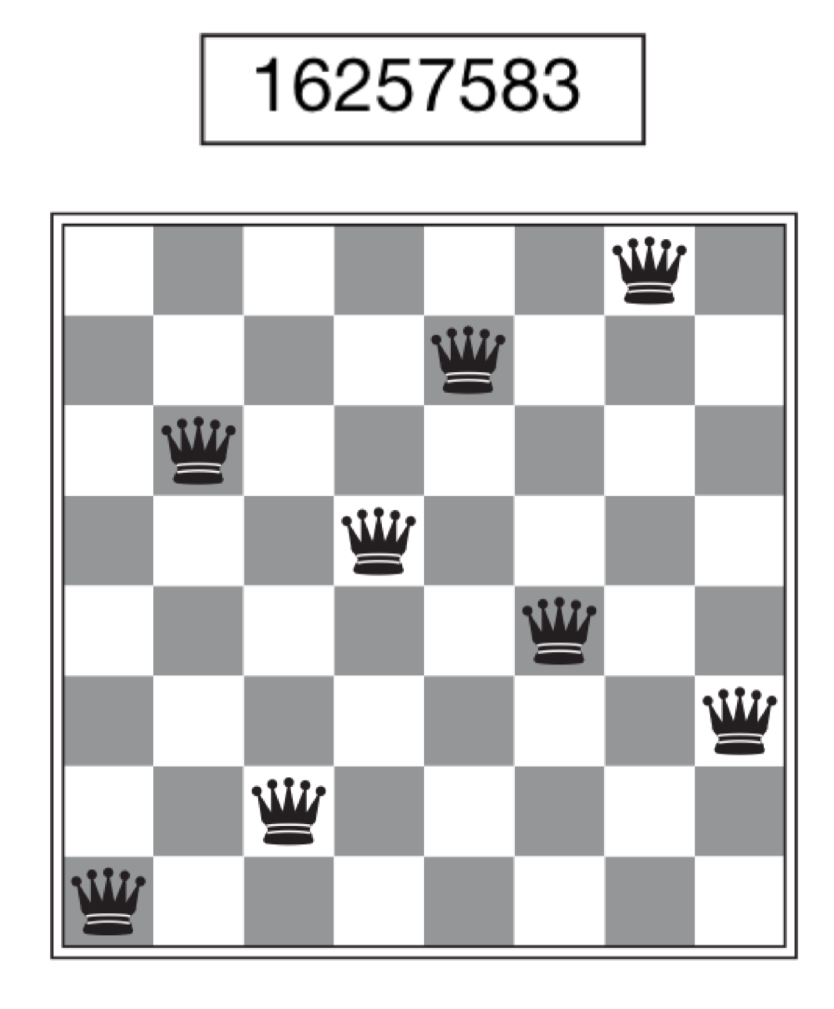
\includegraphics[width=0.3\textwidth]{img/img6.png} \\
    \scriptsize Here we are ordering the genotype by columns. It can also be expressed via rows.
\end{center} \vspace{3.5pt}
Defined the representation of states, each of them is rated by a \textbf{fitness function}, such that the algorithm will take some genotypes for the production of the next 
generation of states. A fitness function should return higher values for better states, so, for the 8-queens problem we use the number of non-attacking pairs of queens. In 
this case, the probability of being choosen for reproducing is directly proportional to the \textbf{fitness score}. \vspace{3.5pt}

According to the fitness probabilities, pairs of genotypes are taken from the population and then combined for the reproduction. Hopefully, if the parent genotypes are great 
solutions, then the offspring generated might be a better solution than before, but it's not guaranteed. For each pair, a \textbf{crossover point} is chosen randomly 
from the position in the string. As in the example introduced, portions of the array representation are swapped. \vspace{3.5pt}

Finally, the offspring generated is subject to a random \textbf{mutation}, one of the digit that composed the array representation is changed; this corresponds to choosing a 
queen randomly and moving it to a random cell. A visual summary on the main steps of genetic algorithms is shown below. \vspace{3.5pt}
\begin{center}
    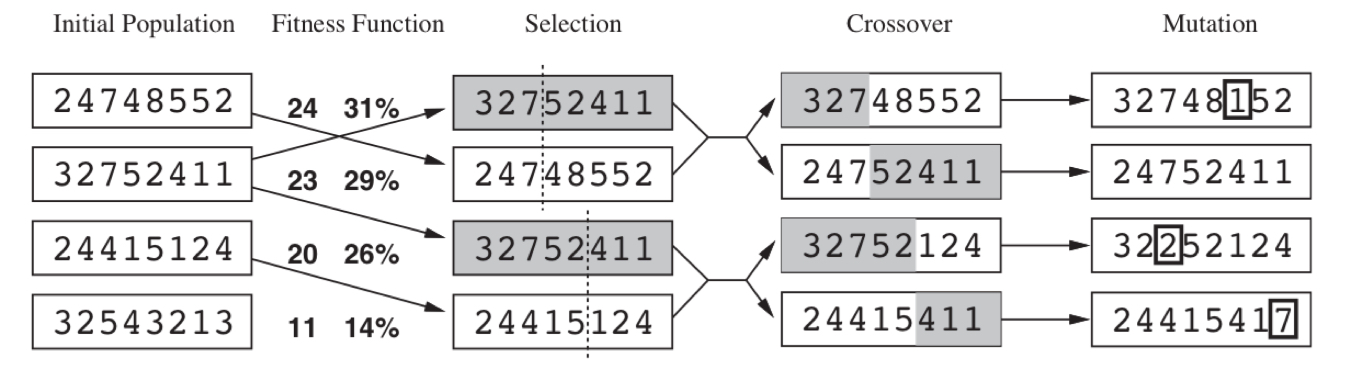
\includegraphics[width=0.9\textwidth]{img/img7.png}
\end{center} \vspace{3.5pt}

Replacing all the population each time a new generation is created, it determines a method that is computationally easier than any other algorithm seen so far; we substitute 
the old population with a new one, and that's it. However, this behavior can cause a major disadvantage: good solutions are not maintained in the new population. Generally, 
to avoid this, the best $n$ individuals from the new and old population are kept, hoping that the next generation can achieve a greater result. \vspace{3.5pt}

Despite genetic algorithms being extremely simple and easy to associate with different types of purposes, they are influenced by two main constraints:
\begin{itemize}
    \renewcommand{\labelitemi}{-}
    \item It can be a little too simple according to the operations performed.
    \item We have to tune a lot of parameters; remember the representation of genotypes, results coming from mutation, permutation and selection or the crossover point.
\end{itemize}
\label{s_4_3}

\section{Summary}
\begin{table}[h!]
    \centering
    \begin{tabularx}{\textwidth}{|p{2.5cm}|X|X|}
        \hline
        Preferable & \bf Local search & \bf Genetic algorithm \\
        \hline
        1. & Neighborhood structures create a correlated search graph. & Solutions can be encoded as composition of states. \\
        \hline
        2. & Computational cost of moves is low. & Computational cost of moves in local search is high. \\
        \hline
        3. & Inventing moves is easy. & It is difficult to design effective neighborhood structures and a way to visit them. \\
        \hline
    \end{tabularx}
\end{table}
\label{s_4_4}

\chapter{Swarm intelligence}
Concerning population based methods, now we explore another type of algorithms known as \textbf{Swarm Intelligence} algorithms.
\begin{definition}
    \textbf{Swarm Intelligence}, briefly SI, is an artificial intelligence technique based around the study of collective behavior in decentralized and self-organized systems.
\end{definition}

A simpler definition expresses Swarm Intelligence algorithms as a set of artificial intelligence methods that rely on \textbf{AI agents}, where each of them is totally autonomus
and independent. So, any agent has its own goals and decision algorithm. \vspace{3.5pt}

The entire swarm, in any kind of algorithm, has this nice feature: we can always examine an emerging behavior that comes from the interactions taken by any single agent\footnote{The \textbf{emerging behavior} does not come from the planning established by the algorithm!}.
Therefore, the key idea about Swarm Intelligence is to take some individuals, that are soo simple, and put them all together, thus defining a quite complex self-organization. \vspace{3.5pt}

Each type of self-organization is based on three major ingredients, as follows:
\begin{itemize}[nosep]
    \renewcommand{\labelitemi}{-}
    \item \textbf{Multiple interactions among agents}. \\ As we said, the organization is composed by some simple agent, and each of them has its own goals and decision algotithm. Putting them together, we are defining a \textbf{multi-agent system}: from the taken interactions we can retrieve an emerging behavior.
    \item \textbf{Positive feedback}. \\ Imitating, with positive feedback, successfull behaviors. 
    \item \textbf{Negative feedback}. \\ Suppose we have a \textit{food source}, for us means a solution with a higher fitness score. If the food is already exhausted, so in the neighborhood of the current solution $N(s)$ nothing is left, we move to somewhere else.
\end{itemize}

We will consider three main algorithms, based on the last intuition defined, which are:
\begin{itemize}[nosep]
    \renewcommand{\labelitemi}{-}
    \item Ant Colony Optimization.
    \item Particle Swarm Optimization.
    \item Artificial Bee Colony Algorithm.
\end{itemize}
\label{c_5}

\section{Ant Colony Optimization}
This type of algorithm is the simpliest and works only for those Bayesian networks that have no given evidences. The idea is to sample each random variable that composed the
network, following its topological order. Note that the probability distribution from which the value is sampled is conditionated on the values already assigned to the 
variable's parents. \vspace{3.5pt}

The algorithm, shown below, generates samples from the prior joint distribution specified by the network. Let's consider a new example for better understanding.
\begin{example}
    i.e. Sampling by sprinkler network. \vspace{3.5pt}

    From the same network, used to understand the first basic concepts about Bayesian networks, we assume the same topological order, such as: \vspace{3.5pt}
    \begin{center}
        $[Cloudy, Sprinkler, Rain, WetGrass]$
    \end{center} \vspace{3.5pt}

    By the sampling algorithm, we have to associate a sample value with each node:
    \begin{enumerate}
        \item $\mathbf{P}(Cloudy)$. \\
        From the initial CPT, the boolean variable has the same probability to assume $True$ or $False$, $\langle 0.5, 0.5\rangle$. In this case, the algorithm gives us 0.1,
        so $Cloudy = True$.
        \item $\mathbf{P}(Sprinkler|Cloudy=True)$. \\
        Again, we know that $P(Sprinkler=True|Cloudy=True) = 0.1$ and $P(Sprinkler=False|Cloudy=True) = 0.9$. The method return us 0.2, so $Sprinkler = False$. 
        \item $\mathbf{P}(Rain|Cloudy=True)$. \\
        Analyzing the CPT, we have $P(Rain=True|Cloudy=True) = 0.8$ and $P(Rain=False|Cloudy=True) = 0.2$. The sample value is 0.7, the boolean value associated is 
        $True$.
        \item $\mathbf{P}(WetGrass|Sprinkler=False, Rain=True)$. \\
        Another time, we use the conditional probability table to see what happens if are given these evidences. Therefore, $P(WetGrass = True|Sprinkler=False, Rain=True) = 0.9$
        and $P(WetGrass=False|Sprinkler=False, Rain=True) = 0.1$, the final value is $True$. 
    \end{enumerate} 
    In this case, \textit{Prior-Sample} return us $\langle t,f,t,t \rangle$
\end{example}
From the previous example, we can compute which is the probability that \textit{Prior-Sample} generates a particular event. First, let $S_{PS}(x_1, \dots, x_n)$ be the probability
that a specific event is generated by the algorithm, then we have:
\begin{center}
    $S_{PS}(x_1, \dots, x_n) = \prod_{i=1}^{n}P(x_i|Parents(X_i))$
\end{center}
so, the probability that a specific event is generated is equal to the product of each conditional probability given the parents of $X_i$. Accordingly to the definition of
\textit{global semantics}, we have:
\begin{center}
    $S_{PS}(x_1, \dots, x_n) = \prod_{i=1}^{n}P(x_i|Parents(X_i)) = P(x_1 \dots x_n)$.
\end{center}
This last observation tell us exactly that the algorithm generates samples from the prior joint distribution! \vspace{3.5pt}

Generally, the answers are computed by counting the actual samples generated. Suppose there are $N$ total samples, and let $N_{PS}(x_1, \dots, x_n)$ be the number of times
the specific event occurs in the set of samples. Then we have:
\begin{center}
    $\lim_{N \rightarrow \infty} \frac{N_{PS}(x_1, \dots, x_n)}{N} = S_{PS}(x_1, \dots, x_n) = P(x_1 \dots x_n)$.
\end{center}
We expect $\frac{N_{PS}}{N}$ to converge to its expected value according to the sampling probability. \vspace{3.5pt}

For instance, consider the previously event: \textit{[t,f,t,t]}. The sampling probability for this event is:
\begin{center}
    $S_{PS}(t,f,t,t) = 0.5 \times 0.9 \times 0.8 \times 0.9 = 0.324$.
\end{center} \vspace{3.5pt}

Hence, we expect $32.4\%$ of the samples to be of this event. That is, estimates derived from \textit{Prior-Sample} are \textbf{consistent}, briefly:
\begin{center}
    $P(x_1 \dots x_n) \approx \frac{N_{PS}(x_1, \dots, x_m)}{N}$
\end{center}
\label{s_5_1}
\end{document}